\chapter{Test dei metodi di spam detection}
\lstset{basicstyle=\small\ttfamily,keywordstyle=\color{black}\bfseries,commentstyle=\color{darkgray},stringstyle=\color{black},showstringspaces=true} 
Nei capitoli precendenti sono stati illustrati vari metodi che di spam detection classificati basandosi sui segnali in ingresso che essi hanno bisogno per poter identificare le pagine web; quindi si hanno tre classi: metodi basati sul contenuto, metodi basati sul grafo e metodi che utilizzano segnali diversi dai primi due. Tra questi metodi ne sono stati presi in esame due: \textit{Trustrank} e \textit{Anti-trust rank}. 

Si è scelto, quindi, di valutare l'efficacia di due  algoritmi \textit{linked base} (\textit{Trustrank} e \textit{Anti-trust rank}) se essi operassero in modo online. Più precisamente i vari test consistono nel verificare quanto questi due algoritmi di tipo offline riescano ad approssimare il loro comportamento se li facessimo operare in modo online ovvero durante la fase di crawling. Le domande che ci poniamo eseguendo questi test su i due algoritmi di spam dection offline (\textit{Trustrank} e \textit{Anti-trus rank}) sono:
\begin{itemize}
 \item possono questi algoritmi essere in grado di operare in modalità online?
 \item durante l'esecuzione in modalità online, quanto riescono ad approssimare il loro comportamento offline?
 \item è conveniente utilizzare questi algoritmi in modalità online?
\end{itemize}

E' doveroso specificare che un algoritmo di spam detection lavora offline se questo viene eseguito dopo l'attività di crawling (e quindi dopo che si ha a disposizione l'intero grafo ottenuto dai collegamenti tra le pagine), mentre un algoritmo di spam detection lavora online se questo viene eseguito durante il processo di crawling e quindi riesce a determinare all'istante se una pagina deve essere considerata spam o non spam. Dal momento che si è scelto di esaminare degli algoritmi \textit{linked base}, e sapendo che questi formulano delle conclusioni sulla natura delle pagine (ovvero se sono spam o non spam) esaminando la struttura dell'intero grafo, è interessante notare come questi si comportino se il grafo su cui fare le valutazioni è incompleto.
%altre considerazioni

Il capitolo è diviso nel seguente modo: nella prima parte verrà illustrato come è stato scelto di simulare il crawler per poter eseguire gli algoritmi offline duratne la fase di crawling; nella seconda parte verrà spiegato come sono stati implementati i test; infine verrano illustrati tutti i test.

\section{Simulazione del crawler}
Per simulare il comportamento di crawler, e quindi eseguire gli algoritmi di \textit{Trustrank} e \textit{Anti-trust rank}, abbiamo implementato una semplice visita sul grafo in ampiezza ovvero una BFS \cite{bfsCormen} (Breadth-First Search). La visita in ampiezza dato un grafo \(G=(V,E)\), dove \(V\) è l'insieme dei vertici del grafo ed \(E\) l'insieme degli archi del grafo, e un vertice \(s\) da cui far partire la visita, scopre tutti i vertici che sono raggiungibili da \(s\). La visita in ampiezza scopre tutti i vertici che si trovano a distanza \(f\) dal vertice di partenza e successivamente scopre i vertici che si trovano a una distanza successiva \(f+1\). In sostanza dato il nodo di partenza \(s\), la visita in ampiezza, scopre tutti i nodi vicini al nodo \(s\) e successivamente per ogni nodo vicino scoperto trova i vicini che non sono ancora stati visitati; questo processo viene iterato finche tutti i nodi del grafo raggiungibili da \(s\) sono visitati. \\
Quindi anziche implementarci l'algoritmo BFS abbiamo utilizzato l'implementazione definita nel framework WebGraph. In particolare è stata utilizzata la classe ``ParallelBreadthFirstVisit'' che esegue una visita in ampiezza utilizzando il parallelismo derivato dai processori multicore.

\section{I test}
Come gia introdotto lo scopo dei test consiste che dato un algoritmo di spam detection che opera in modo offline valutare le sue prestazioni se operasse in modo online. Oltre tutto abbiamo scelto due algoritmi \textit{linked base} quali \textit{Trustrank} e \textit{Anti-trust rank} questo significa che l'algoritmo opererà su un grafo del web incompleto, all'inizio del crawling, fino ad arrivare ad operare sull'intero grafo alla fine del crawling.

\begin{figure}
\centering
 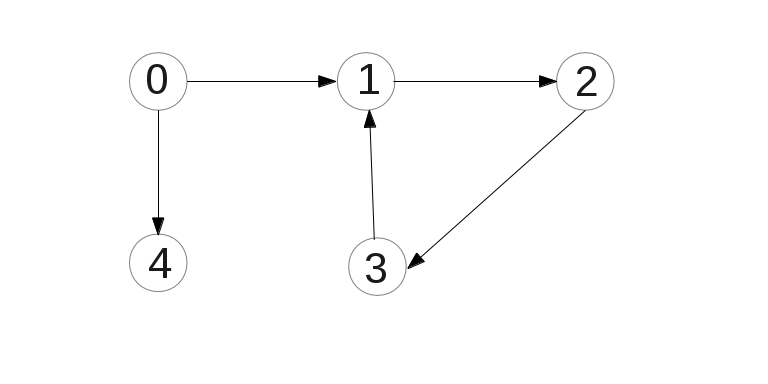
\includegraphics{immagini/test/grafoComp}
 \caption{Esempio di grafo}
 \label{fig:grafoComp}
\end{figure}

Quasi tutti i test seguono uno stesso schema; viene eseguito \textit{Trustrank} (e \textit{Anti-trust rank}) sul grafo completo, e lo indicheremo con \(t\) (\textit{Anti-trust rank} sarà indicato con \(a\)), successivamente viene eseguita la BFS (ovvero la visita in ampiezza) con nodo sorgente \(s\) e quindi si ricava la coda \(q\) dei nodi visitati a partire da \(s\); dopo di che si calcola \textit{Trustrank} (e \textit{Anti-trust rank}) sul grafo ricavati lungo la visita in ampiezza formato, quindi, da un sottoinsieme di nodi \(q\), il risultato lo indicheremo con \(\hat{t}_i\) (\textit{Anti-trust rank} sarà indicato con \(\hat{a}_i\)) dove \(i\) è il numero di nodi presi in considerazione dalla coda \(q\). Questo processo viene iterato incrementando sempre di più l'intervallo \(i\) finché non si arriva alla fine della coda \(q\) dei nodi visitati partendo dal nodo \(s\). Dopo aver calcolato \(t\) e \(\hat{t}_i\) sono due vettori si possono valutare tramite la Tau di Kendall e indicheremo con \(\tau(t,\hat{
t}_i)\) la Tau di Kendall per \(t\) e \(\hat{t}_i\)  (e quindi \(\tau(a,\hat{a}_i)\) sarà la Tau di Kendall per \(a\) e \(\hat{a}_i\)). Ad esempio in figura \ref{fig:grafoComp} è rappresentato il grafo completo su cui verra calolato \(t\) e \(a\) mentre in figura \ref{fig:grafo3} è rappresentato il grafo ricavato dalla BFS eseguita sul grafo precedente partendo dal nodo 1; se si considerano tutti i nodi lungo la visita il vettore di \textit{trustrank} sarà \(\hat{t}_3\) mentre quello di \textit{anti-trust rank} sara \(\hat{a}_3\)..

 \begin{figure}
\centering
 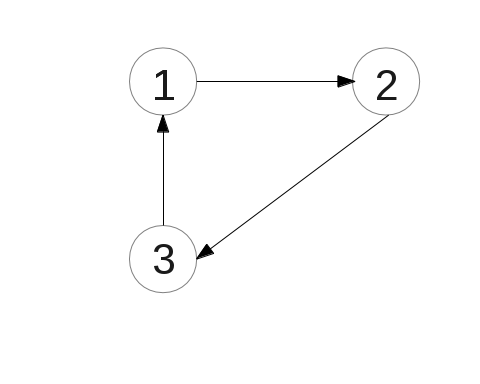
\includegraphics{immagini/test/grafo3}
 \caption{Esempio di grafo ricavato tramite una BFS a partire dal nodo 1 del grafo in figura \ref{fig:grafoComp}.}
 \label{fig:grafo3}
\end{figure}
A ogni indice del  vettore di \textit{Trustrank} \(t\) e del vettore di \textit{Anti-trust rank} \(a\) corrisponderà un nodo è il valore del vettore per un dato indice indica il valore di \textit{Trustrank} e \textit{Anti-trust rank} del nodo del grafo. In figura \ref{fig:tVettore} è illustrato un esempio del vettore di \textit{trustrank} calcolato sull'intero grafo e in figura \ref{fig:aVettore} è illustrato un esempio del vettore di \textit{anti-trust rank} calcolato sull'intero grafo. 
Nell'esempio in figura \ref{fig:tVettore} si nota che il vettore \(t\) di \textit{trustrank} ha lunghezza 5, quindi il grafo sarà composto da 5 nodi dove ad ogni nodo è associato il valore di \textit{trustrank}. Le stesse considerazioni valgono per l'esempio in figura \ref{fig:aVettore} dove il vettore di \textit{anti-trust rank} è ha lunghezza 5 e quindi l'algoritmo opererà su un grafo composto da 5 nodi.

\begin{figure}
\centering
 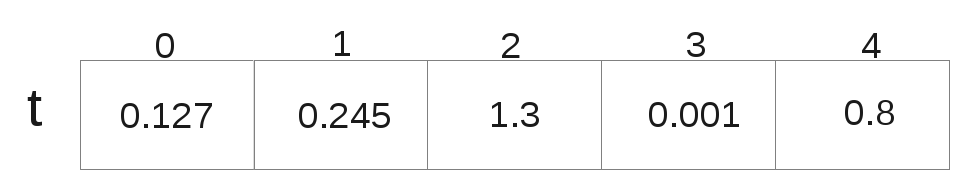
\includegraphics{immagini/test/trustVettore}
 \caption{Esempio del vettore di trustrank calcolato sull'intero grafo}
 \label{fig:tVettore}
\end{figure}
\begin{figure}
\centering
 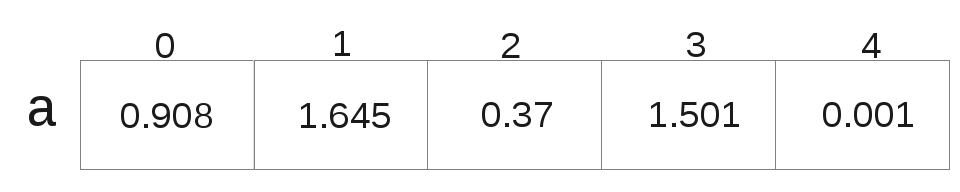
\includegraphics{immagini/test/immagineAntiTrust}
 \caption{Esempio del vettore di anti-trust rank calcolato sull'intero grafo}
 \label{fig:aVettore}
\end{figure}

A differenza dei vettori \(t\) e \(a\) (\textit{trustrank} eseguito sull'intero grafo e \textit{anti-trust rank} sull'intero grafo) , dove ad ogni indice (cioè ad ogni nodo) è associato un valore di \textit{trustrank} e \textit{anti-trust rank} , i vettori \(\hat{t}_i\) e \(\hat{a}_i\) non avranno per ogni indice un valore associato. Più precisamente, sapendo che \(\hat{t}_i\) e \(\hat{a}_i\) sono calcolati durante l'esecuzione di una BFS allora a ogni passo ci saranno ancora dei nodi da visitare per cui non è possibile calcolare i valori di \textit{trustrank} e \textit{anti-trust rank}, perciò con l'avanzamento della visita in ampieza sempre più nodi avranno associato un valore di \textit{trustrank} e \textit{anti-trust rank}. Vale quindi che \(\hat{t}_{i+1}\) avrà molti più nodi per cui è stato calcolato \textit{trustrank} rispetto a \(\hat{t}_i\) (lo stesso comportamento si riscontra per \textit{anti-trust rank}). Inoltre non è detto che dopo aver terminato la visita in ampiezza, partendo da un nodo \(s\),
 si sia visitato tutto il grafo (ovvero che \(s\) può raggiungere tutti i nodi del grafo) perciò in questo caso \(\hat{t}_i\) e \(\hat{a}_i\) avranno un numero minore di nodi per cui è calcolato \textit{trustrank} e \textit{anti-trust rank} rispetto a \(t\) e \(a\).\\
Dal momento che la Tau di Kendall tra due vettori, per essere eseguita, richiede che i due vettori abbiano la stessa lunghezza allora bisogna gestire i casi in cui i nodi del grafo temporaneo (ottenuto ad ogni intervallo di nodi visitato tramite la visita in ampiezza) non abbiano associato un valore. Per gestire tale problema si è scelto di considereare i soli nodi compresi nel grafo temporaneo. Ad esempio in figura \ref{fig:tBFSmodoB} viene illustrato il caso in cui eseguendo la BFS dal nodo 1, i nodi 0 e 4 rimangano senza aver assegnato un valore di \textit{trustrank}. Quindi gli indici 0 e 4 del vettore \(t\) non sono inclusi nel vettore \(\hat{t}_3\) questo implica che ci deve essere una corrispondenza tra gli indice del vettore \(t\) e quelli del vettore \(\hat{t}_3\) (in figura \ref{fig:tBFSmodoB} l'indice 0 del vettore \(\hat{t}_3\) corrisponde all'indice 1 del vettore \(t\), l'indice 1 al indice 2 ed infine l'indice 2 all'indice 3).  Si inoltre nota che il vettore \(\hat{t}_3\) ha lunghezza inferiore 
al vettore \(t\). Inoltre il calcolo della Tau di Kendall sara tra il vettore \(t\) formato dai soli indici compresi nel vettore \(\hat{t}_i\) e dal vettore \(\hat{t}_i\). Quindi  nella valutazione  il vettore \(t\) dovra essere ristretto alla lunghezza del vettore \(\hat{t}_i\) e quindi dovranno essere eliminati gli indici del vettore \(t\) che non sono inclusi nel vettore \(\hat{t}_i\).
\begin{figure}
\centering
 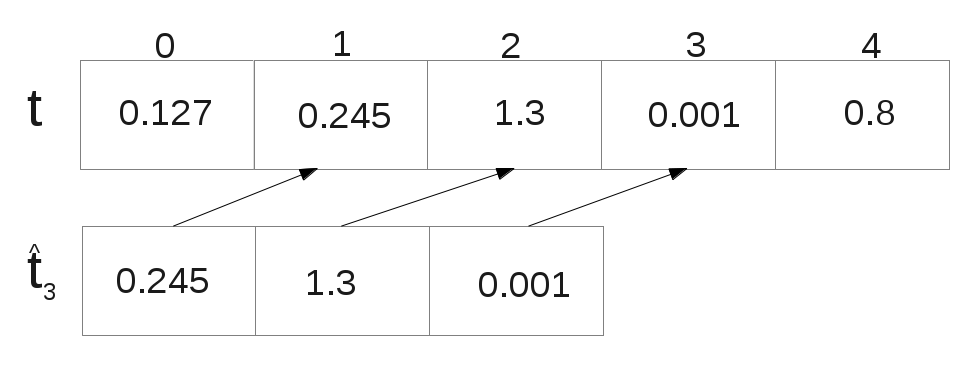
\includegraphics{immagini/test/tBFSmodoB}
 \caption{Esempio del vettore di trustrank calcolato su una porzione di grafo.}
 \label{fig:tBFSmodoB}
\end{figure}
Un altro metodo che può essere utilizzato è quello di assegnare ad ogni indice dei vettori \(\hat{t}_i\) e \(\hat{a}_i\) non ancora visitati il valore 0.0. Ad esempio prendendo in considerazione il grafo in figura \ref{fig:grafoComp} e ipotizzando di eseguire una BFS a partire dal nodo 1 e di aver visitato i nodi 2 e 3 quindi se calcoliamo \textit{trustrank} e \textit{anti-trust rank} sul sottografo ricavato dai nodi visitati, i nodi 0 e 4 avranno associato i valori 0.0 (usando il metodo \textit{Modo\_A}), tale esempio è illustrato in figura \ref{fig:tBFSmodoA} e in figura \ref{fig:aBFSmodoA}. Questa metodo però è poco significativo in quanto vengono introdotti dei valori non veritieri che producono rumore, e quindi non verrà preso in considerazione.
\begin{figure}
\centering
 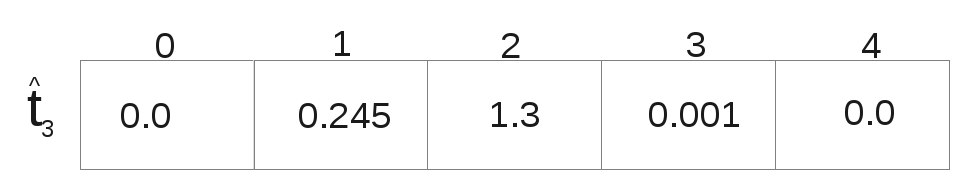
\includegraphics{immagini/test/tBFSmodoA}
 \caption{Esempio del vettore di trustrank calcolato su una porzione di grafo a cui viene assegnato il valore 0.0 ai nodi non visitati.}
 \label{fig:tBFSmodoA}
\end{figure}
\begin{figure}
\centering
 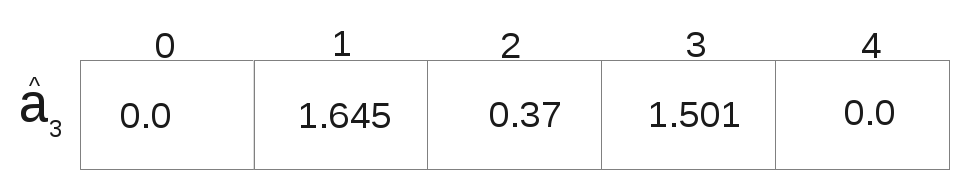
\includegraphics{immagini/test/aBFSmodoA}
 \caption{Esempio del vettore di anti-trust rank calcolato su una porzione di grafo a cui viene assegnato il valore 0.0 ai nodi non visitati.}
 \label{fig:aBFSmodoA}
\end{figure}

I test saranno, quindi, cosi strutturari:
\begin{itemize}
 \item Test numero 1. Si confronta \textit{trustrank} sul grafo completo con \textit{trustrank} calcolato su una porzione di grafo. Lo stesso si fa per \textit{anti-trust ran}.
 \item Test numero 2. Si confrontano i solo nodi etichettati spam del vettore di  \textit{trustrank} sul grafo completo con  i soli nodi etichettati spam del vettore di \textit{trustrank} calcolato su una porzione di grafo. Nel caso di \textit{anti-trust rank} si  confrontano i nodi etichettati come non spam.
 \item Test numero 3. Si calcola \textit{trustrank} sul grafo completo ottenuto eseguendo la visita partendo da un nodo \(s\) e si confronta con \textit{trustrank} eseguito a ogni passo delle visita ma si imposta un seedset diverso formato dagli ultimi \(n\) nodi della vista. Viene applicato lo stesso metodo per \textit{anti-trust rank}.
 \item Test numero 4. Si esegue la BFS a partire dal nodo \(s\) e per ogni passo si calola la media dei valori di \textit{trustrank} dei soli nodi che sappiamo essere non spam e la media dei valori di \textit{Trustrank} dei soli nodi spam. Quindi si calcola la differenza tra le due medie. Lo stesso metodo verrà applicato per l'analisi dell'algoritmo di \textit{anti-trust rank}.
 \end{itemize}
 
\section{Test 1}
 Questo test calcola la distanza, tramite della Tau di Kendall denominata \(T_t\), tra il vettore \(t\) di \textit{trustrank} ricavato sull'intero grafo e il vettore \(\hat{t}_i\) di \textit{trustrank} calcolato sul grafo ricavato dai nodi visitati lungo una visita in ampiezza con nodo sorgente \(s\). Inoltre viene eseguto lo stesso procedimento per quanto riguarda \textit{anti-trust rank} ovvero si calcolano le distanze, sempre utlizzando una Tau di Kendall che denomineremo \(T_a\),  tra il vettore di \(a\) di \textit{anti-trust rank} ottenuto dal grafo completo e il vettore \(\hat{a}_i\)  caloato sul grafo ricavato dai nodi visitati lungo  un visita in ampiezza con nodo sorgente \(s\). Dal dataset sono impostati come nodo sorgente della BFS due nodi: il nodo 62 etichettato come non spam e il nodo 112 etichettato come spam. Inoltre per il calcolo di \textit{trustrank} sull'intero grafo viene utilizzato come seedset l'insieme di pagine del dataset WEBSPAM-UK2007 etichettate come non spam mentre per il calcolo di \textit{trustrank} sul grafo ottenuto dai nodi visitati durante la BFS il seedset sarà formato dalle pagine visitate che sono etichettate come non spam nel dataset WEBSPAM-UK2007. Per il calolo di \textit{anti-trust rank} sull'intero grafo, invece, il seedset sarà composto dalle pagine etichettate come spam nel dataset WEBSPAM-UK2007 mentre il seedset di \textit{anti-trust rank} calcolato sul grafo ottenuto dai nodi visitati dalla BFS sarà formato dai soli nodi visitati che sono etichettati come spam.

In figura \ref{fig:test1trustModoB62} e in figura \ref{fig:test1trustModoB112} sono rappresentati rispettivamente i grafici delle Tau di Kendall \(T_{t62}\) e \(T_{t112}\), per il cacolo delle distanze tra il vettore \(t\) calcolato sull'intero grafo e il vettore \(\hat{t}_i\) calcolato sul grafo ottenuto dai nodi visitati lungo una visita in ampiezza con nodo sorgente nel primo caso 62 e nel secondo con nodo sorgente 112.  Sull'asse delle ascisse è rappresentato il numero di nodi che sono stati visitati attraverso la BFS e quindi il numero di nodi del grafo su cui viene calcolato \(\hat{t}_i\) dove \(i\) è appunto il numero di nodi presi in considerazione, mentre sull'asse delle ordinate è rappresentato il valore della Tau di Kendall tra il vettore \(t\) e \(\hat{t}_i\).\\
I due grafici sono molto simili è quindi il calcolo di \(\hat{t}_i\) non dipende dal nodo da cui sorgente della visita in ampiezza. Il valore di Tau di Kendall uguale ad 1 si ha quando la BFS ha visitato solamente il nodo di partenza, quindi  il vettore \(t\) avrà un solo indice (che fa riferimento al nodo sorgente) e il vettore \(\hat{t}_1\) avrà anche esso un solo indice (il quale fa riferimento al nodo sorgente) perciò  la Tau di Kendall tra i due vettori ritorna un valore uguale ad 1; è facile intuire che questo valore non è influente nella valutazione ma è un risultato dovuto al fatto che si calcolcola la Tau di Kendall su vettori composti da un unico elemento, quindi i valori significativi sono i successici.\\
Dopo che la visita entra in profondità il valore delle Tau di Kendall \(T_{t62}\) e \(T_{t112}\)  scendono dastricamente a circa 0.7 per poi aumentare fino a circa 1 tanto più la visita in ampiezza scopre i nodi del grafo; tale comportamento indica che la distanza tra il vettore \(t\) e \(\hat{t}_i\) dipende dal numero di nodi visitati tramite la visita in ampiezza. 

 \begin{figure}
\centering
 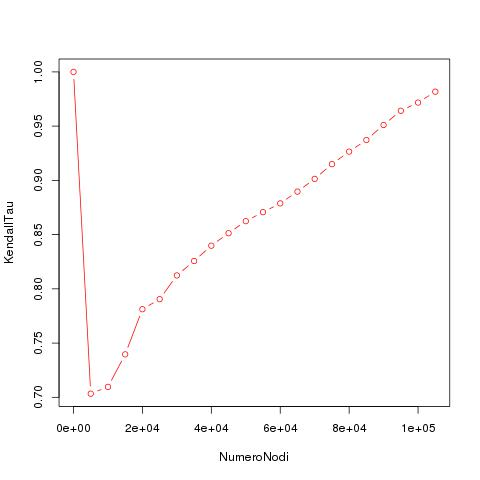
\includegraphics[height=9cm]{immagini/test1/trustranktestMode1_62}
 \caption{Test numero 1 (trustrank, 62). Calcolo della distanza dei vettori tra trustrank calcolato sull'intero grafo e trustrank calcolato sul grafo ricavato dai nodi visitati lungo una BFS partendo dal nodo 62.}
 \label{fig:test1trustModoB62}
\centering
 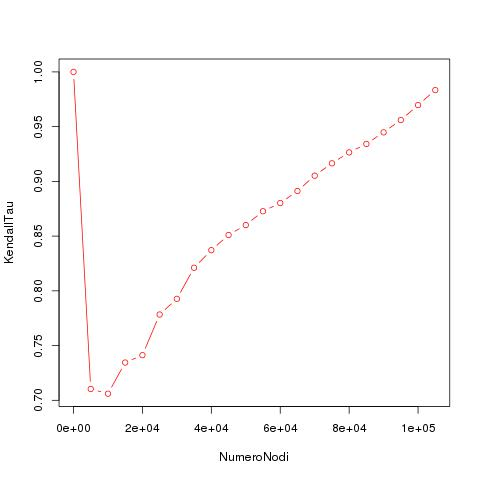
\includegraphics[height=9cm]{immagini/test1/trustranktestMode1_112}
 \caption{Test numero 1 (trustrank, 112). Calcolo della distanza dei vettori tra trustrank calcolato sull'intero grafo e trustrank calcolato sul grafo ricavato dai nodi visitati lungo una BFS partendo dal nodo 112.}
 \label{fig:test1trustModoB112}
\end{figure}

Eseguendo lo stesso test per valutare la distanza tra il vettore \(a\) di \textit{anti-trust rank} calcolato sull'intero grafo e il vettore \(\hat{a}_i\) calcolato sul grafo ottenuto dai nodi visitati durante una visita in ampiezza si nota che i risultati sono presocchè uguali ai precedenti due test. In particolare in figura \ref{fig:test1antitrustModoB62} è rappresentato il grafico della Tau di Kendal \(T_{a62}\) che mette a confronto il vettore \(a\) con il vettore \(\hat{a}_i\) dove la BFS ha come nodo sorgente 62 mentre in figura \ref{fig:test1antitrustModoB112} è rappresentato il grafico della Tau di Kendall \(T_{a112}\) che mette a confronto il vettore \(a\) con il vettore \(\hat{a}_i\) dove la BFS ha nodo sorgente 112; sull'asse delle ascisse è rappresentao il numero di nodi che sono visitati durante la BFS mentre sulle ordinate il corrispondente valore di Tau di Kendall tra il vettore di \(a\) calcolato sull'intero grafo e il vettore \(\hat{a}_i\) calcolato sul grafo ricavato dai nodi visitati attraverso una BFS a diversi passi, quindi \(i\) sarà uguale al numero dei nodi visitati ad un certo istante. Rispetto al test di \textit{trustrank} usando \textit{anti-trust rank} si nota che i grafici (senza considerare il primo valore per lo stesso motivo dei due test precedenti) hanno un andamento quasi logaritmico dove si ha come valore iniziale di Tau di Kendall 0.75 e come utlimi valori (stazionari) 0.95. Infatti un fattore evidente è che la Tau di Kendall tende a non superare il 0.95 per gli ultimi nodi incontrati nella BFS.

 \begin{figure}
\centering
 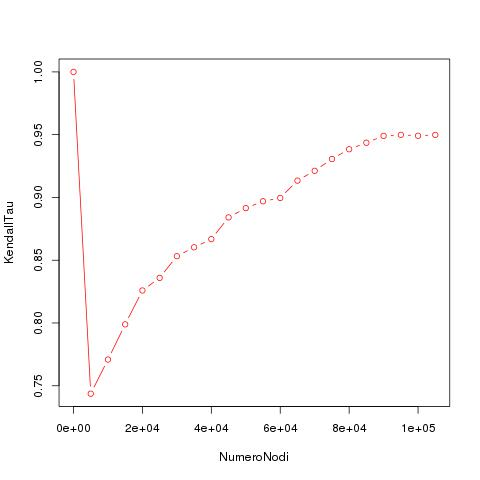
\includegraphics[height=9cm]{immagini/test1/antiTrustrankTestMode1_62}
 \caption{Test numero 1 (anti-trust rank, 62). Calcolo della distanza dei vettori tra anit-trust rank calcolato sull'intero grafo e anti-trust rank calcolato sul grafo ricavato dai nodi visitati lungo una BFS parteneo dal nodo 62.}
 \label{fig:test1antitrustModoB62}
\centering
 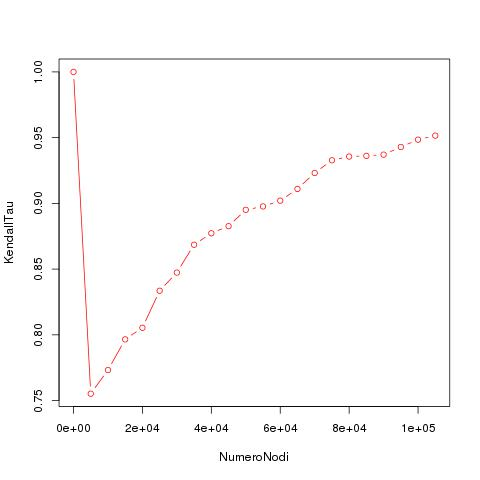
\includegraphics[height=9cm]{immagini/test1/antiTrustrankTestMode1_112}
 \caption{Test numero 1 (anti-trust rank, 112). Calcolo della distanza dei vettori tra anit-trust rank calcolato sull'intero grafo e anti-trust rank calcolato sul grafo ricavato dai nodi visitati lungo una BFS parteneo dal nodo 112.}
 \label{fig:test1antitrustModoB112}
\end{figure}

In figura \ref{fig:test1coplot62} sono riportati in un unico grafico i grafici rappresentati in figura \ref{fig:test1trustModoB62} relativo a \(T_{t62}\) e del  grafico \ref{fig:test1antitrustModoB62} relativo a \(T_{a62}\); in rosso è rappresentato il grafico raffigurante \(T_{t62}\) tra \textit{trustrank} calcolato sull'intero grafo e \textit{trustrank} calcolato sul grafo ottenuto dai nodi visitati a diversi passi di una BFS con nodo sorgente 62 mentre in verde è rappresentato il grafico  rappresentante \(T_{a62}\) tra \textit{anti-trust rank} calcolato sull'intero grafo e \textit{anti-trust rank} calcolato sul grafo ottenuto dai nodi visitati a diversi passi di una BFS con nodo sorgente 62. Quello che evince è che \(T_{a62}\) applicata al vettore \(a\) e \(\hat{a}_i\) cresce più velocemente rispetto a \(T_{t62}\) applicata a   \(t\) e \(\hat{t}_i\) ma che dopo la visita di circa 80000 \(T_{t62}\) assume valori più alti rispetto a \(T_{a62}\); infatti come avevamo detto i valori di \(T_{a62}\) tendono a fermarsi intorno a 0.95.\\
Tale comportamento tra \(T_{t62}\) e \(T_{a62}\) indica perciò che \textit{trustrank} eseguito online è più efficace di \textit{anti-trust rank} nel approssimare il loro comportamento offline ma solo dopo che sono stati visitati molti nodi mentre \textit{anti-trust rank} online riesce ad approssimare bene il suo comportamento anche se eseguito su un numero esiguo di nodi dell'intero grafo. Quindi  tra \textit{trustrank} e \textit{anti-trust rank} il miglior metodo per essere utilizzato in modalità online è \textit{anti-trust rank} perché tende ad approssimare fin da subito il comportamento offline anche avendo pochi nodi. Infatti il grafico in figura \ref{fig:test1coplot62} indica che \textit{anti-trust rank} eseguito durante la fase di crawling ritorna un vettore dove i valori tendono ad avvicinarsi rapidamente ai valore del vettore se \textit{anti-trust rank} fosse eseguito in modalità offline. Le stesse valutazioni valgono tra il confronto dei due grafici in figura \ref{fig:test1trustModoB112} relativo a \(T_{t112}\) e \ref{fig:test1antitrustModoB112}  relativo a \(T_{a112}\) illustrato in figura \ref{fig:test1coplot112} dove in rosso è rappresentata la Tau di Kendall  tra \textit{trustrank} calcolato sull'intero grafo e \textit{trustrank} calcolato sul grafo ottenuto dai nodi visitati a diversi passi di una BFS con nodo sorgente 112 mentre in verde è rappresentato il la Tau di Kendall tra \textit{anti-trust rank} calcolato sull'intero grafo e \textit{anti-trust rank} calcolato sul grafo ottenuto dai nodi visitati a diversi passi di una BFS con nodo sorgente 112.

 \begin{figure}
\centering
 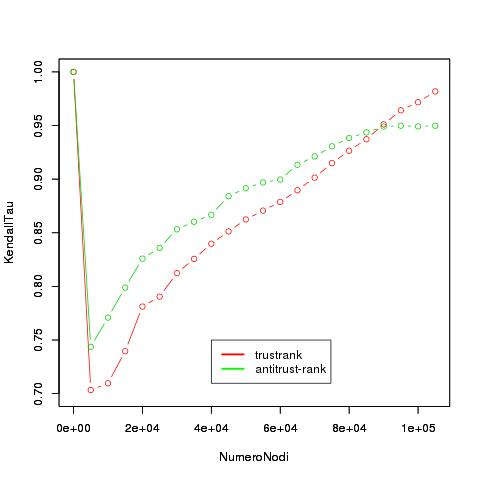
\includegraphics[height=9cm]{immagini/test1/coplotTrustAnti_62}
 \caption{Plotting del grafico \ref{fig:test1trustModoB62} e del  grafico \ref{fig:test1antitrustModoB62}}
 \label{fig:test1coplot62}
\centering
 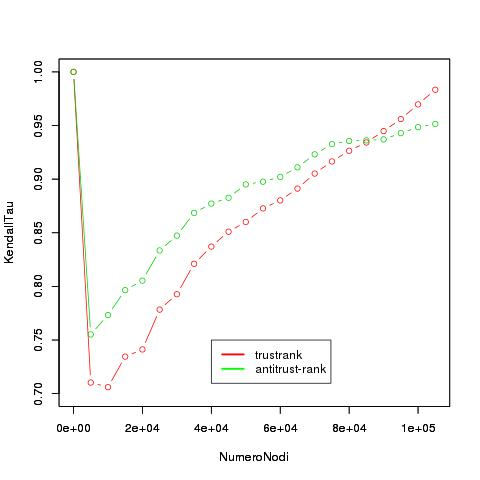
\includegraphics[height=9cm]{immagini/test1/coplotTrustAnti_112}
 \caption{Plotting del grafico \ref{fig:test1trustModoB112} e del  grafico \ref{fig:test1antitrustModoB112}}
 \label{fig:test1coplot112}
\end{figure}

\section{Test 2}
Il test consiste nel valutare la distanza tra due vettori, il vettore \(t\) di \textit{trustrank} calcolato sull'intero grafo e il vettore \(\hat{t}_i\) calcolato sul grafo ottentuto dai nodi visitati durante un visita in ampiezza; quindi la distanza viene calcolata ogni qual volta il numero di indici, del vettore \(\hat{t}_i\), a cui è possibile associare un valore aumenta  di un certo intervallo ovvero  quando la BFS visita un intervallo di nodi stabilito adentrandosi sempre di più nel grafo. Il test cosi descritto è simile al \textit{Test numero 1} ma differentemente del precedente in questo test nel determinare la distanza tra i due vettori si esaminano i soli indici che fanno riferimento ai nodi etichettati come spam. Ugualmente il test viene effettuato per valutare \textit{anti-trust rank} ma in questo caso vengono confrontati i soli nodi indici dei due vettore \(a\) e \(hat{a}_i\) che fanno riferimento a nodi etichettati come non spam.

Anche per questo test nella valutazione di \textit{trustrank} è stato usato come seedset l'insieme dei nodi etichettati non spam del dataset WEBSPAM-UK2007 mentre per \textit{anti-trustrank} è stato usto come seedset l'insieme dei nodi spam del dataset WEBSPAM-UK2007.

\subsection{Modo\_A}

\begin{figure}
\centering
 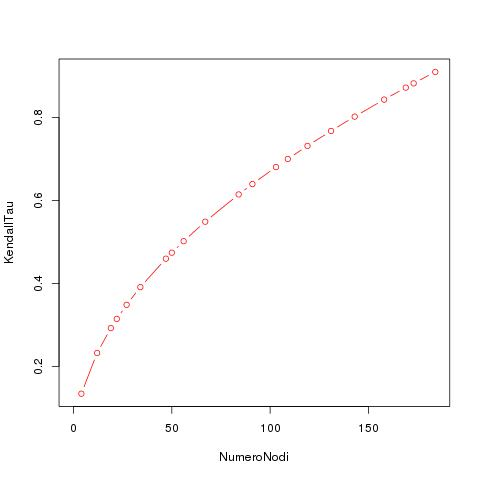
\includegraphics[height=9cm]{immagini/test2/trustrankBadNodesTestMode0_62}
 \caption{Test numero 2 (trustrank, 62). Calcolo della distanza dei vettori, usando il Modo\_A, tra trustrank calcolato sull'intero grafo e trustrank calcolato sul grafo ricavato dai nodi visitati lungo una BFS partendo dal nodo 62 prendendo in considerazione i soli nodi spam. }
 \label{fig:test2trustModoA62}
\centering
 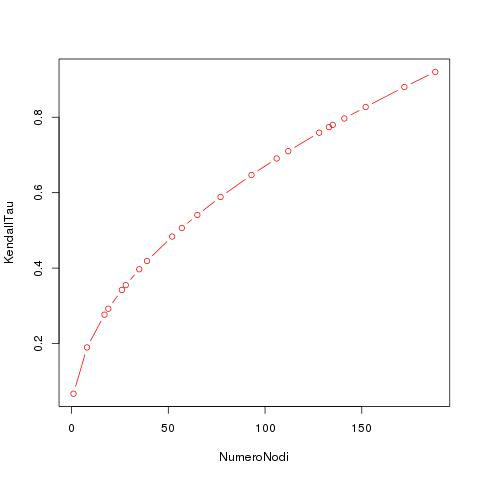
\includegraphics[height=9cm]{immagini/test2/trustrankBadNodesTestMode0_112}
 \caption{Test numero 2 (trustrank, 112). Calcolo della distanza dei vettori, usando il Modo\_A, tra trustrank calcolato sull'intero grafo e trustrank calcolato sul grafo ricavato dai nodi visitati lungo una BFS partendo dal nodo 112 prendendo in considerazione i soli nodi spam.}
 \label{fig:test2trustModoA112}
\end{figure}

Il test calcola la distanza tra i soli indici del vettore \(t\) di \textit{trustrank}, ottenuto sull'analisi dell'intero grafo, che fanno riferimento a nodi spam e i gli indici del vettore \(\hat{t}_i\) di \textit{trustrank}, ottenuto dall'analisi del grafo ricavato ogni intervallo di nodi visitato tramite una visita in ampiezza, che fanno riferimento a nodi spam.

I risultati del test effettuato su \textit{trustrank}, usando il \textit{Modo\_A}, sono illustrati in figura \ref{fig:test2trustModoA62} e in figura \ref{fig:test2trustModoA112}; nel primo grafico il nodo sorgente della visita in ampiezza, che viene utilizzata per costruire il grafo temporaneo ogni intervallo di nodi visitati e su cui viene calcolato \(\hat{t}_i\) ad ogni intervallo, è il nodo 62 mentre nel secongo grafico il nodo è 112.  Sull'asse delle ascisse sono rappresentati il numero di nodi che sono spam tra quelli che vengono visitati tramite la visita in ampiezza mentre sull'asse delle ordinate è rappresentato il valore della Tau di Kendall tra i nodi spam del vettore \(t\) e i nodi spam del vettore \(\hat{t}_i\), calcolata a ogni intervallo di nodi visitati tramite la visita in ampiezza.\\
Entrambi i grafici evidenziano che all'aumentare di nodi visitati attraverso la visita in ampiezza e quindi all'aumentare del grafo temporaneo su cui viene calcolato \(\hat{t}_i\), il vettore \(\hat{t}_i\) ha i valore dei nodi spam che sono molto più vicini ai vaolori de nodi spam del vettore \(\hat{t}_i\); infatti si nota che verso la fine della visita la Tau di Kendall dei valori dei nodi del vettore \(t\) con i valori dei nodi spam del vettore \(\hat{t}_i\) è circa 1. 

Quanto descritto per l'analisi di \textit{trustrank} vale per \textit{anti-trust rank}. In figura in figura \ref{fig:test2antitrustModoA62} e in figura \ref{fig:test2antitrustModoA112} sono illustrati i grafici relativi alla Tau di Kendall tra i gli indici dei nodi non spam del vettore \(a\) di \textit{anti-trust rank}, calcolato sull'intero grafo, e gli indici  del vettore \(\hat{a}_i\) di \textit{trustrank}, ottenuto dall'analisi del grafo ricavato ogni intervallo di nodi visitato tramite una visita in ampiezza, che fanno riferimento a spam; Nel primo grafico il nodo sorgente della visita in ampiezza è 62 mentre nel secondo è 112. Sull'asse delle ascisse sono rappresentati il numero di nodi non spam tra i nodi visitati tramite la visita in ampiezza mentre sull'asse mentre sull'asse delle ordinate è rappresentato il valore della Tau di Kendall tra nodi non spam del vettore \(a\) e i nodi non spam del vettore \(\hat{a}_i\).\\
La  Tau di Kendall tra i nodi non spam del vettore \(a\) e del vettore \(\hat{a}_i\) cresce sempre di più con l'aumentare dei nodi visitati attrverso la visita in ampiezza fino ad arrviare a circa uno quando quasi tutto il grafo è stato visitato e quindi il valore di \(\hat{a}_i\) riprodurrà quasi fendelemnte i valori del vettore \(a\). Questo fattore è duvuto al fatto che il grafo temporaneo ricavato dai nodi visitati tramite la visita in ampiezza sarà sempre più simile al grafo completo tanto più la visita entra in profondità e quindi \textit{anti-trust rank} calcolato su tale grafo riprodurrà sempre più con maggiore affidabilità i valori calcolati sull'intero grafo.


\begin{figure}
\centering
 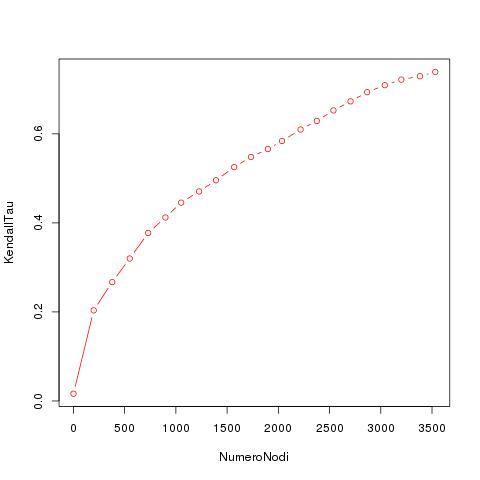
\includegraphics[height=9cm]{immagini/test2/antiTrustraktGoodNodesTestMode0_62}
 \caption{Test numero 2 (anti-trust rank, 62). Calcolo della distanza dei vettori, usando il Modo\_A, tra anti-trust rank calcolato sull'intero grafo e anti-trust rank calcolato sul grafo ricavato dai nodi visitati lungo una BFS partendo dal nodo 62 prendendo in considerazione i soli nodi non spam. }
 \label{fig:test2antitrustModoA62}
\centering
 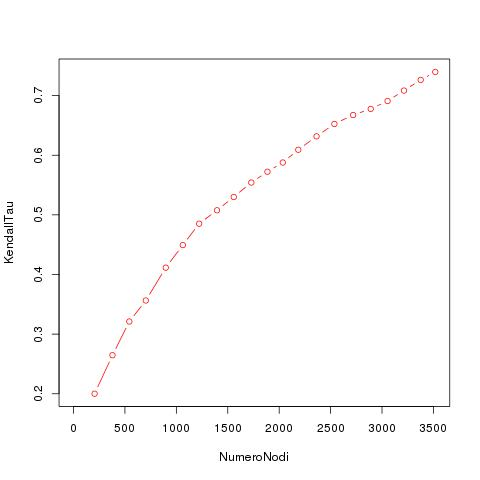
\includegraphics[height=9cm]{immagini/test2/antiTrustraktGoodNodesTestMode0_112}
 \caption{Test numero 2 (anti-trust rank, 62). Calcolo della distanza dei vettori, usando il Modo\_A, tra anti-trust rank calcolato sull'intero grafo e anti-trust rank calcolato sul grafo ricavato dai nodi visitati lungo una BFS partendo dal nodo 112 prendendo in considerazione i soli nodi non spam. }
 \label{fig:test2antitrustModoA112}
\end{figure}

\subsection{Modo\_B}
Anche nel \textit{Modo\_B} il test determina la distanza tra i soli indici del vettore \(t\) di \textit{trustrank} (o dei soli indici del vettore \(a\) nel caso di \textit{anti-trust rank}), ottenuto sull'analisi dell'intero grafo, che fanno riferimento a nodi spam e i gli indici del vettore \(\hat{t}_i\) di \textit{trustrank} (o dei soli indici del vettore \(\hat{a}_i\) nel caso di \textit{anti-trust rank}), ottenuto dall'analisi del grafo ricavato ogni intervallo di nodi visitato tramite una visita in ampiezza, che fanno riferimento a nodi spam.

\begin{figure}
\centering
 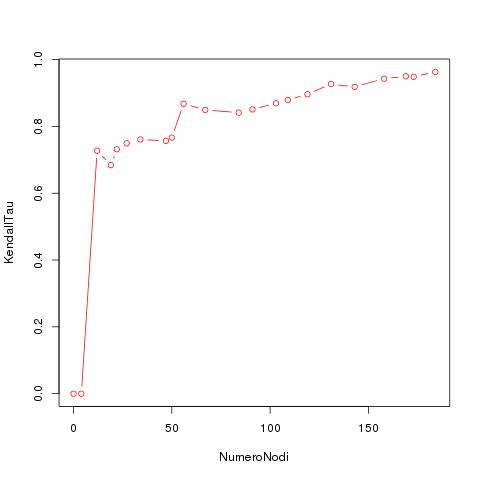
\includegraphics[height=9cm]{immagini/test2/trustrankBadNodesTestMode1_62}
 \caption{Test numero 2 (trustrank, 62). Calcolo della distanza dei vettori, usando il Modo\_B, tra trustrank calcolato sull'intero grafo e trustrank calcolato sul grafo ricavato dai nodi visitati lungo una BFS partendo dal nodo 62 prendendo in considerazione i soli nodi spam. }
 \label{fig:test2trustModoB62}
\centering
 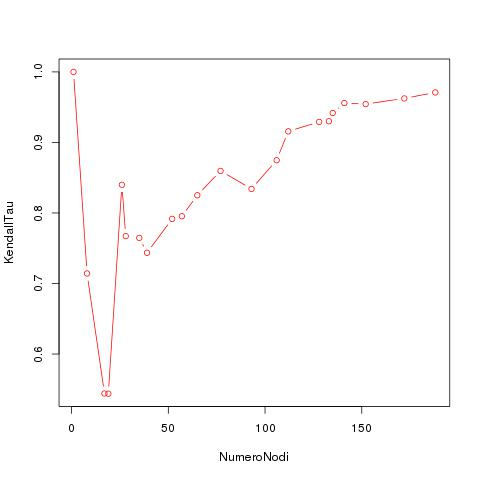
\includegraphics[height=9cm]{immagini/test2/trustrankBadNodesTestMode1_112}
 \caption{Test numero 2 (trustrank, 112). Calcolo della distanza dei vettori, usando il Modo\_B, tra trustrank calcolato sull'intero grafo e trustrank calcolato sul grafo ricavato dai nodi visitati lungo una BFS partendo dal nodo 112 prendendo in considerazione i soli nodi spam.}
 \label{fig:test2trustModoB112}
\end{figure}

In figura \ref{fig:test2trustModoB62} è rappresentato il grafico di tale esperimento dove il nodo sorgente della visita in ampiezza è 62 dove sull'asse delle ascisse è rappresentato il numero di nodi spam tra tutti i nodi visitati e sull'asse delle ordinate la Tau di Kendall calcolato a ogni intervallo di nodi visitati (spam e non spam). Dal momento che si sta eseguendo il test nel \textit{Modo\_B} ci si aspetta che (come per il test numero 1) il primo valore della Tau di Kendall (ovvero quando la BFS ha visitato solo il nodo sorgente) sia 1 ma visto che si stanno prendendo i soli nodi spam in questo caso dato che il nodo sorgente è non spam il nodo è scartato è quindi i vettore \(t\) e \(\hat{t}_i\) sono vuoti differentemente dal \textit{Modo\_A} dove ai nodi del vettore \(\hat{t}_i\) che risultavano non spam veniva assegnato il valore 0.0. Dopo di che l'andamento del grafico cresce rapidamente fino a circa 0.7 per poi variare gradualemnte fino a circa 1.0.\\
Se il nodo sorgente della visita in ampiezza è 112 la Tau di Kendall calcolata  per ogni intervallo di nodi visitati tramite la visita in ampiezza è rappresentato in figura \ref{fig:test2trustModoB112} dove sull'asse delle ascisse è rappresentato il numero di nodi spam tra tutti i nodi visitati e sull'asse delle ordinate la Tau di Kendall calcolato a ogni intervallo di nodi visitati . In questo caso il primo valore della Tau di Kendall è 1 questo perché essendo che il nodo 112 è un nodo spam e il primo valore lo si ha quando il grafo temporaneo su cui viene calcolato \(\hat{t}_i\) è composto da 1 solo nodo (ovvero il nodo 112 perchè è l'inizio della visita) il vettore \(\hat{t}_i\) sarà composto da un univo indice e di conseguenza (dal momento che stiamo utilizzando il \textit{Modo\_B}) anche il vettore \(t\) sarà ridotto ad avere quel solo indice per calcolre la distanza. Dopo di che l'andamento della Tau di Kendall varia tra circa 0.5 e 1.\\
Gli stessi test sono stati applicati per valutare \textit{anti-trust rank}; in figura \ref{fig:test2antitrustModoB62} è illustrato il grafico relativo al calcolo della distanza tra il vettore \(a\) e il vettore \(\hat{a}_i\) prendendo in considerazione i soli nodi non spam e la visita in ampiezza ha nodo sorgente 62, mentre in figura \ref{fig:test2antitrustModoB112} è illustrato lo stesso test ma cambia il nodo sorgente della visita in ampiezza che è 112. Sull'asse delle ascisse è rappresentato il numero di nodi non spam tra tutti i nodi visitati e sull'asse delle ordinate la Tau di Kendall calcolato a ogni intervallo di nodi visitati. Nel primo grafico si nota che a differenza del test su \textit{trustrank} con nodo sorgente, della BFS, 62 il primo valore della Tau di Kendall, ovvero quando la visita in ampiezza ha visitato il solo nodo sorgente e quindi il grafo temporaneo è formato dal solo nodo 62, è 1 perchè essendo che in questo caso si esaminano i nodi non spam tale nodo non viene rigettatto ma viene 
esaminato e quindi nel vettore \(\hat{a}_i\) vi è un solo valore relativo al nodo 62 e questo vale per il vettore \(a\) che viene ridimensionato (ed ecco il perchè del valore 1 che assume la Tau di Kendall). Dopo di che i valori variano da circa 0.75 a 0.95.
\begin{figure}
\centering
 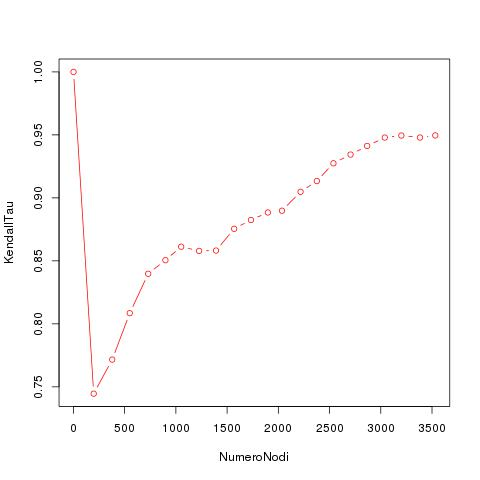
\includegraphics[height=9cm]{immagini/test2/antiTrustraktGoodNodesTestMode1_62}
 \caption{Test numero 2 (anti-trust rank, 62). Calcolo della distanza dei vettori, usando il Modo\_B, tra anti-trust rank calcolato sull'intero grafo e anti-trust rank calcolato sul grafo ricavato dai nodi visitati lungo una BFS partendo dal nodo 62 prendendo in considerazione i soli nodi non spam. }
 \label{fig:test2antitrustModoB62}
\centering
 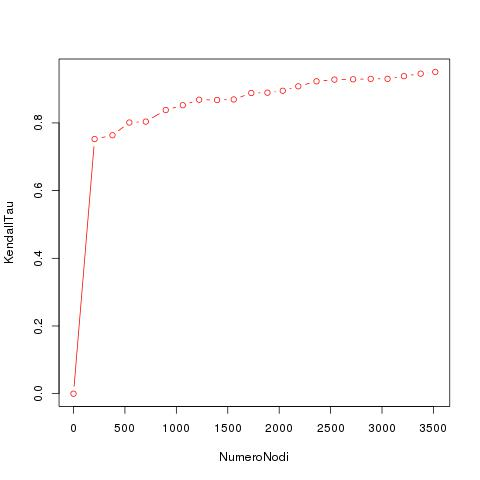
\includegraphics[height=9cm]{immagini/test2/antiTrustraktGoodNodesTestMode1_112}
 \caption{Test numero 2 (anti-trust rank, 62). Calcolo della distanza dei vettori, usando il Modo\_B, tra anti-trust rank calcolato sull'intero grafo e anti-trust rank calcolato sul grafo ricavato dai nodi visitati lungo una BFS partendo dal nodo 112 prendendo in considerazione i soli nodi non spam. }
 \label{fig:test2antitrustModoB112}
\end{figure}
Il secondo grafico mentre ha come primo valore di Tau di Kendall 0, questo perchè il grafo temporaneo è formato al primo passo è formato dal solo nodo 112 e quindi dal momento che 112 è un nodo spam viene rigettato e non esamenito. Perciò in questo caso sia il vettore \(a\) che il vettore \(\hat{a}_i\) avranno lunghezza zero fino al mometo in cui la visita in ampiezza non incotra dei nodi non spam. Infatti nei passi successivi il grafico varia da circa 0.8 a circa 1.
 

 
